\chapter{Model hrozieb}
\label{ch:threat-model}

Model hrozieb určuje, čo sa chráni, kto útočí a ktorý prvok má ktorý útok zastaviť. Útoky sú klasifikované metódou STRIDE (časť~\ref{sec:stride}) a každý z nich má v repozitári automatizovaný test.

\section{Systém a aktíva}

Chráneným systémom je aplikácia Bookinfo~\cite{istio-bookinfo} na clustri z troch uzlov (kapitola~\ref{ch:design}). Graf volaní je
\texttt{productpage} $\rightarrow$ \texttt{details} a \texttt{productpage} $\rightarrow$ \texttt{reviews} $\rightarrow$ \texttt{ratings} $\rightarrow$ \texttt{mongodb}; pody sú rozmiestnené tak, že každé volanie prechádza medzi uzlami. Aktíva sú v tabuľke~\ref{tab:assets}.

\begin{table}[ht!]
  \centering
  \caption{Chránené aktíva}
  \label{tab:assets}
  \footnotesize
  \renewcommand{\arraystretch}{1.15}
  \begin{tabularx}{\textwidth}{@{}>{\raggedright\arraybackslash}p{4.6cm}>{\raggedright\arraybackslash}X@{}}
    \toprule
    Aktívum & Kde sa nachádza \\
    \midrule
    Hodnotenia (MongoDB) & pod \texttt{mongodb}; riadenie prístupu je v MongoDB predvolene vypnuté~\cite{mongodb} a Bookinfo ho nezapína, takže jedinou kontrolou prístupu je sieťová dosiahnuteľnosť \\
    Recenzie a hodnotenia počas prenosu & HTTP a protokol MongoDB medzi podmi na rôznych uzloch \\
    Kubernetes API (stav clustra, Secrets) & API server na riadiacom uzle, dosiahnuteľný z podov \\
    Tokeny ServiceAccountov & predvolene pripojené do každého podu \\
    \bottomrule
  \end{tabularx}
\end{table}

Hranice dôvery ležia medzi podmi navzájom (v tom istom namespace), medzi uzlami na sieti uzlov a medzi podom a API serverom.

\section{Model útočníka}

Útočník má jednu z troch pozícií (tabuľka~\ref{tab:attackers}, obrázok~\ref{fig:testbed}). Aktívny útok typu man-in-the-middle na sieti uzlov sa netestuje.

\begin{table}[ht!]
  \centering
  \caption{Pozície útočníka}
  \label{tab:attackers}
  \footnotesize
  \renewcommand{\arraystretch}{1.15}
  \begin{tabularx}{\textwidth}{@{}>{\raggedright\arraybackslash}p{3.2cm}>{\raggedright\arraybackslash}X>{\raggedright\arraybackslash}X@{}}
    \toprule
    Útočník & Pozícia & Schopnosti \\
    \midrule
    Kompromitovaný frontend & spustenie kódu v \texttt{productpage}, verejne dostupnom frontende & ľubovoľné nástroje so sieťovou identitou podu a pripojenými prihlasovacími údajmi \\
    Pozorovateľ siete & na sieti medzi uzlami & pasívny záznam prevádzky medzi uzlami \\
    Tvorca podov & smie vytvárať pody v namespace aplikácie, napríklad cez uniknutý prístup CI alebo vývojára & volí labely, image, vloženie sidecaru a ľubovoľný ServiceAccount namespace \\
    \bottomrule
  \end{tabularx}
\end{table}

\section{Útoky}

Tabuľka~\ref{tab:attacks} uvádza útoky, ich kategórie STRIDE a prvok, ktorý ich má zastaviť. Útoky neoprávnená operácia a kompromitovaná služba predpokladajú útočníka v pode \texttt{reviews}: má platnú identitu aj povolenú sieťovú cestu k \texttt{ratings}. V teste beží ako ephemeral container~\cite{k8s-ephemeral-containers} v skutočnom pode \texttt{reviews}, takže zdieľa jeho sieťovú identitu a v mesh aj jeho sidecar.

\begin{table}[ht!]
  \centering
  \caption{Útoky, kategórie STRIDE a očakávaný ochranný prvok}
  \label{tab:attacks}
  \footnotesize
  \renewcommand{\arraystretch}{1.15}
  \begin{tabularx}{\textwidth}{@{}>{\raggedright\arraybackslash}p{2.7cm}>{\raggedright\arraybackslash}X>{\raggedright\arraybackslash}p{2.7cm}>{\raggedright\arraybackslash}p{1.4cm}>{\raggedright\arraybackslash}p{2.6cm}@{}}
    \toprule
    Útok & Opis & Útočník & STRIDE & Zastaví \\
    \midrule
    Laterálny pohyb & frontend číta databázu a volá backend, ktorý nikdy nepoužíva & kompromitovaný frontend & E, I, T & segmentácia siete \\
    Odpočúvanie siete & záznam prevádzky podov medzi uzlami & pozorovateľ siete & I (T) & šifrovanie medzi uzlami alebo mTLS medzi službami \\
    Podvrhnutie identity & podvrhnutý pod skopíruje dôveryhodný label \texttt{app=reviews} a volá \texttt{ratings}; tri varianty v tabuľke~\ref{tab:spoofing} & tvorca podov & S & podľa variantu \\
    Neoprávnená operácia & kompromitovaný \texttt{reviews} volá \texttt{ratings} metódou, ktorú nepotrebuje (zápis \texttt{POST /ratings/\{id\}}) & útočník v \texttt{reviews} & E, T & L7 autorizácia: od identity \texttt{reviews} iba \texttt{GET /ratings/*} \\
    Kompromitovaná služba & kompromitovaný \texttt{reviews} číta hodnotenia vlastnou platnou identitou po povolenej ceste & útočník v \texttt{reviews} & I & nič (obmedzenie riešenia) \\
    Zneužitie ServiceAccount tokenu & token ServiceAccountu podu použitý voči API serveru & kompromitovaný frontend & S, E, I & segmentácia siete (token sa nepripája, cesta k API serveru chýba), RBAC \\
    \bottomrule
  \end{tabularx}
\end{table}

Popretie (\emph{repudiation}) sa netestuje; čiastočne ho pokrývajú záznamy tokov Hubble od konfigurácie so segmentáciou siete a prístupové logy Envoy v mesh. Odopretie služby je mimo rozsahu projektu.

\subsection{Varianty podvrhnutia identity}

Labely volí ten, kto pod vytvára, takže nie sú identitou, a segmentácia siete im napriek tomu dôveruje. Identitou v mesh je ServiceAccount, no tvorca podov môže zvoliť ľubovoľný ServiceAccount namespace. Samotné mTLS preto nezastaví podvrhnutý pod, ktorý sa do mesh zapojí. Tabuľka~\ref{tab:spoofing} uvádza tri varianty útoku.

\begin{table}[ht!]
  \centering
  \caption{Varianty podvrhnutia identity}
  \label{tab:spoofing}
  \footnotesize
  \renewcommand{\arraystretch}{1.15}
  \begin{tabularx}{\textwidth}{@{}>{\raggedright\arraybackslash}p{2.6cm}>{\raggedright\arraybackslash}p{3.3cm}>{\raggedright\arraybackslash}p{2.4cm}>{\raggedright\arraybackslash}X@{}}
    \toprule
    Variant & Podvrhnutý pod & Zastaví & Prečo \\
    \midrule
    Mimo mesh & bez sidecaru, SA \texttt{default} & mTLS medzi službami (\texttt{STRICT}) & nemá certifikát, nešifrovaná prevádzka je odmietnutá \\
    S iným ServiceAccountom & v mesh, SA \texttt{default} & L7 autorizácia & má platný certifikát (je autentizovaný), ale nie povolenú identitu \\
    S ukradnutým ServiceAccountom & v mesh, SA \texttt{bookinfo-reviews} & nič & nerozlíšiteľný od \texttt{reviews}; vyžaduje admission control alebo RBAC na vytváranie podov a použitie SA (mimo rozsahu) \\
    \bottomrule
  \end{tabularx}
\end{table}

\subsection{Priradenie kontrol pri zneužití ServiceAccount tokenu}

Segmentácia siete pridáva dva nezávislé prvky: NetworkPolicy a nepripájanie tokenu. Aby bol každý výsledok priradený práve jednému prvku, test zneužitia ServiceAccount tokenu sa skladá zo štyroch kontrol (tabuľka~\ref{tab:token}). Ani jeden z prvkov nezaťažuje dátovú cestu, takže meranie réžie segmentácie siete neovplyvňujú.

\begin{table}[ht!]
  \centering
  \caption{Kontroly pri zneužití ServiceAccount tokenu a prvok, ktorý o nich rozhoduje}
  \label{tab:token}
  \footnotesize
  \renewcommand{\arraystretch}{1.15}
  \begin{tabularx}{\textwidth}{@{}>{\raggedright\arraybackslash}X>{\raggedright\arraybackslash}X@{}}
    \toprule
    Kontrola & Rozhoduje (od konfigurácie so segmentáciou siete) \\
    \midrule
    Token je pripojený v pode & \texttt{automountServiceAccountToken: false} \\
    API server je dosiahnuteľný (anonymne, bez tokenu) & default-deny pre odchádzajúcu prevádzku \\
    Požiadavka s tokenom je autentizovaná & chýbajúci token (zastavila by ju aj default-deny) \\
    Čítanie Secrets & RBAC (zamietnuté vo všetkých konfiguráciách vrátane konfigurácie bez ochrany) \\
    \bottomrule
  \end{tabularx}
\end{table}

\section{Vrstvy ochrany}

Obrázok~\ref{fig:scenario-layers} ukazuje, ako jednotlivé vrstvy postupne zužujú množinu útočníkov, ktorí sa dostanú k hodnoteniam. Segmentácia siete prepustí každý pod s povoleným labelom, mTLS medzi službami každý pod s identitou mesh a L7 autorizácia každý workload s povoleným ServiceAccountom. Zvyšné riziko, legitímna identita v rukách útočníka, žiadna sieťová vrstva neodstráni.

\begin{figure}[ht!]
  \centering
  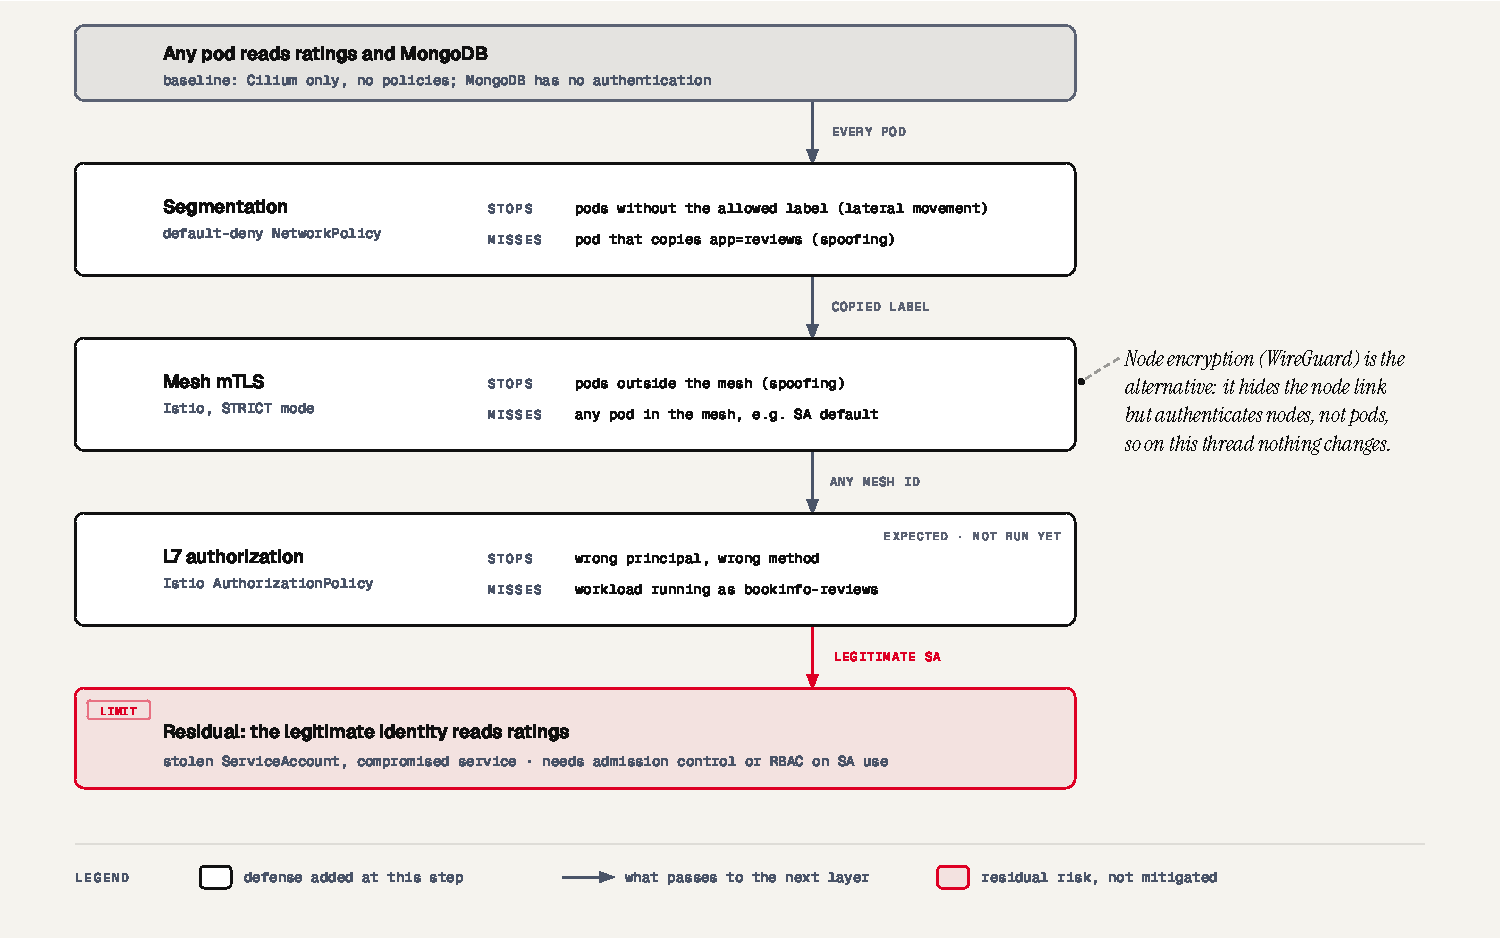
\includegraphics[width=\textwidth]{../figures/scenario-layers.pdf}
  \caption{Čo zastaví ktorá vrstva na ceste k hodnoteniam a zvyškové riziko. Šifrovanie medzi uzlami je alternatívou k mTLS medzi službami; autentizuje uzly, nie pody, a na tejto ceste nič nemení.}
  \label{fig:scenario-layers}
\end{figure}
